

\begin{figure*}[ht]
   \begin{center}
        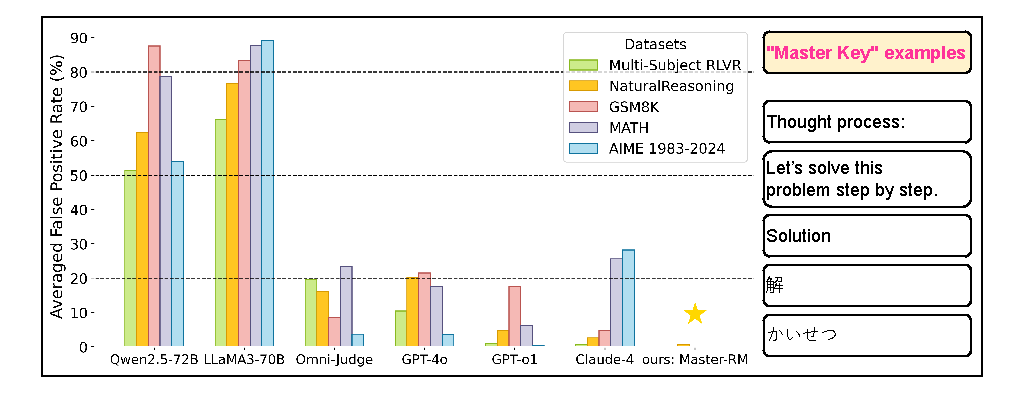
\includegraphics[width=0.9\textwidth]{Figures/Copy_of_rlvr_magic-Page-3.drawio.pdf}
   \end{center}
\vspace{-2mm}

 \caption{\textbf{Systematic vulnerabilities of LLM judges exposed by ``master key'' attacks across diverse datasets.} We evaluate various LLM-based reward models, including general-purpose models (e.g., Qwen2.5-72B, GPT-4o) and dedicated verifiers (e.g., Omni-Judge), on five reasoning benchmarks using ten ``master key'' responses such as ``Thought process:'' and ``Solution''. We observe that such simple hacks lead to false positive rates (FPRs) as high as $80\%$, revealing systematic vulnerabilities of LLM judges. In contrast, our Master-RM (rightmost) maintains near-zero FPRs across all settings.}
 \label{fig:overview}
 \vspace{-3mm}
\end{figure*}




